\chapter{Tehnici de ultimă oră}

Domeniul procesării și generării de sunete și unde sonore a avansat foarte mult în ultimii ani. Tehnicile și metodologiile recente folosesc predominant modele bazate pe rețele neuronale, cu straturi de diverse tipuri.

Unele rețele sunt capabile să genereze muzică din partituri, gramatici sau MIDIuri \cite{dong2017museganmultitracksequentialgenerative}, fie prin producerea de date în același format \cite{dong2017museganmultitracksequentialgenerative}, sau în format de undă sonoră în mod direct.

Alte rețele sunt capabile să genereze muzica în mod direct \cite{li2025jen1textguideduniversalmusic}, preluând o undă sonoră în format digital și generând altă undă sonoră. Deseori acest tip de rețele necesită foarte multe resurse pentru a fi antrenate și folosite.

În această secțiune vor fi prezente o selecție de modele de învățare automată ce au avansat domeniul generării de muzică folosind inteligență artificială.

\section{MuseGAN}

Dong et al. au propus MuseGAN \cite{dong2017museganmultitracksequentialgenerative} drept o soluție pentru generarea de muzică. Arhitectura acestui model presupun două rețele neuronale - o rețea discriminatoare și una generatoare - ce sunt în competiție, similar cum a fost descris în articolul ``\textit{Generative Adversarial Networks}'' (Goodfellow et al.) \cite{goodfellow2014generativeadversarialnetworks}. Cele două rețele sunt compuse din straturi secvențiale de rețele convoluționale. 

\begin{figure}[H]
    \centering
    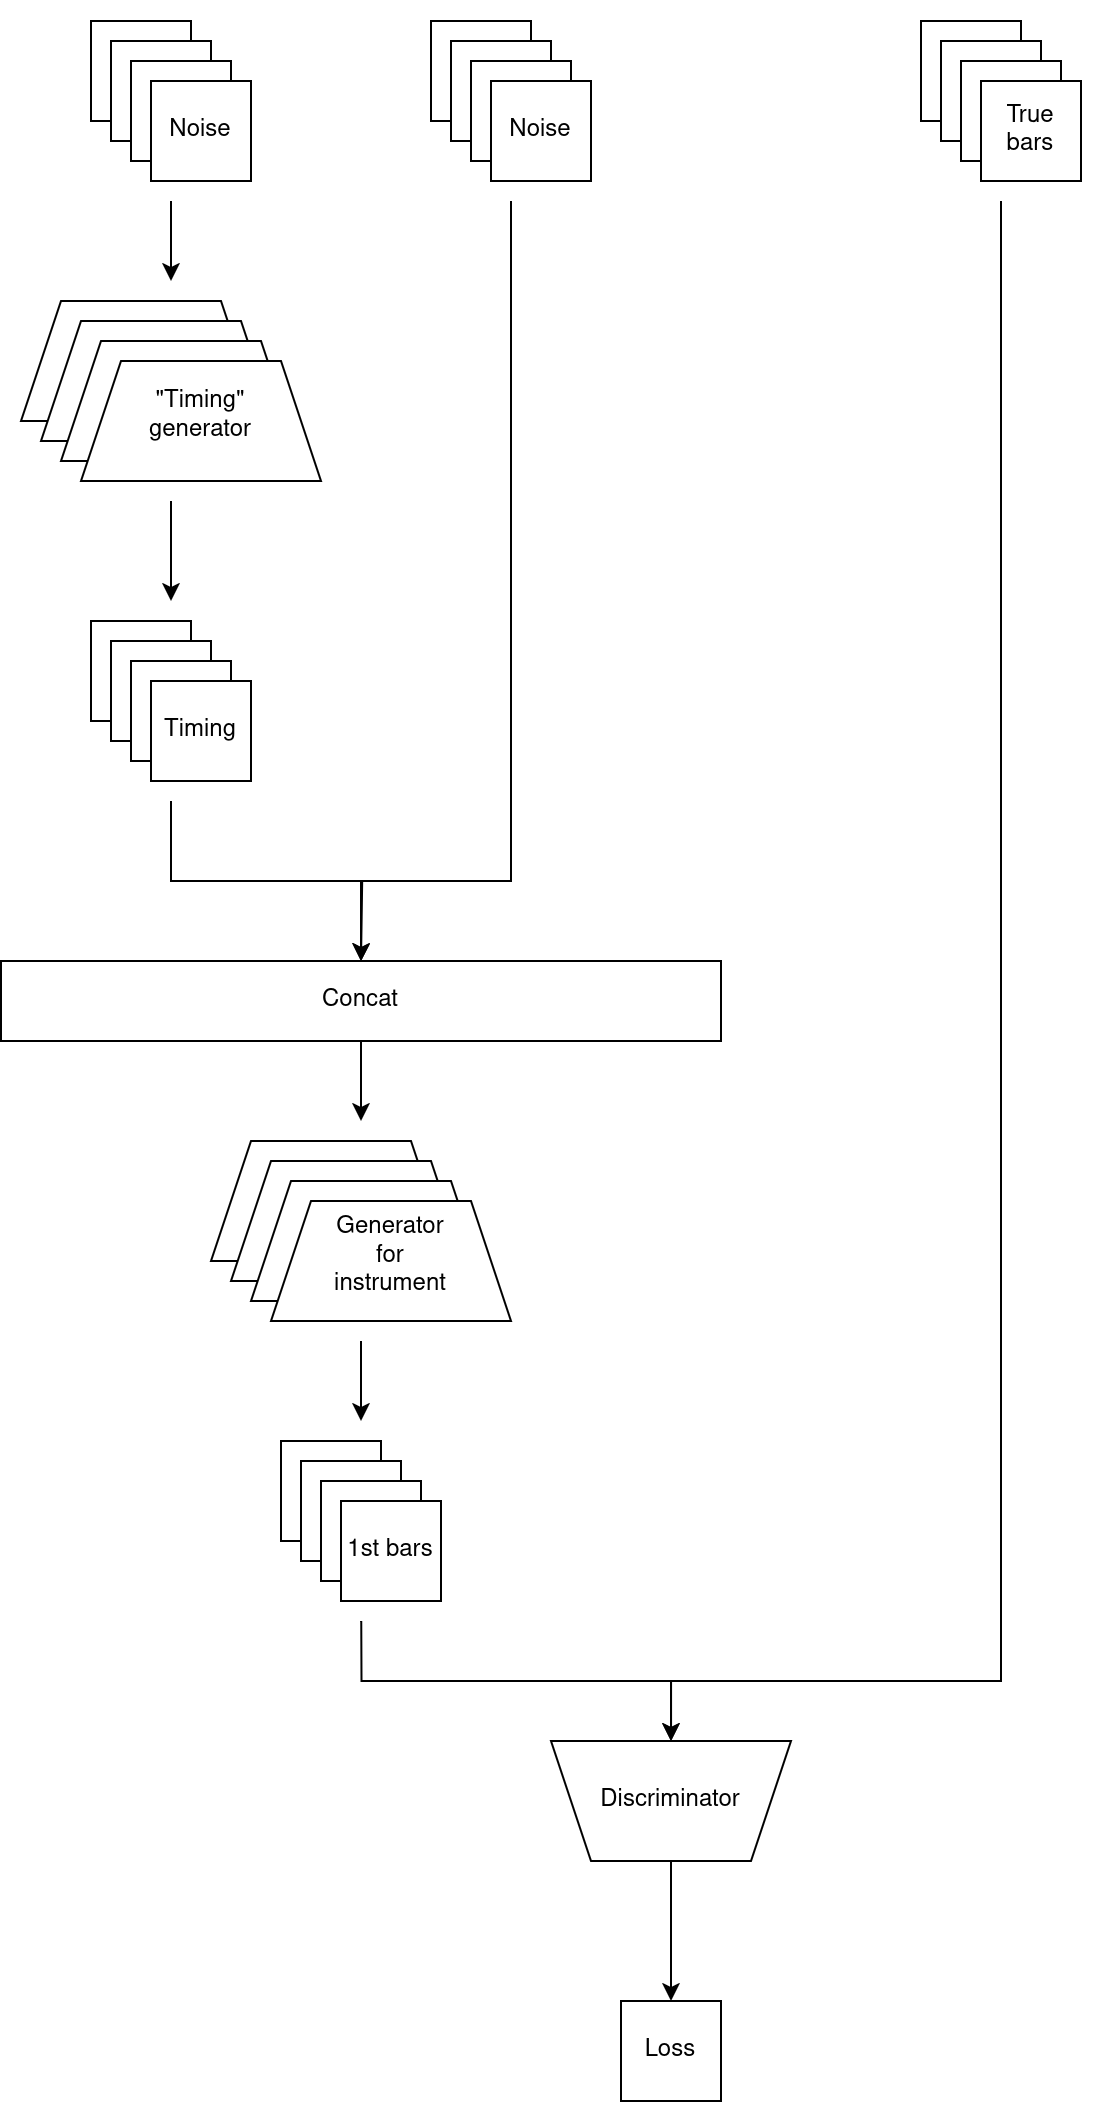
\includegraphics[height=8cm]{musegan.architecture.png}
    \caption{Arhitectura modelului MuseGAN}
    \label{musegan-architecture}
\end{figure}

Discriminatorul modelului este compus dintr-o rețea neuronală convoluțională simplă, ce are ca scop distingerea intrărilor din setul de date real și al intrărilor generate de către generator. Generatorul modelului este compus din două rețele convoluționale. Prima rețea are ca scop generarea structurilor de timp ale unei piese, iar cea de-a doua are ca scop generarea de piano-rolls pentru un anumit instrument.

Autorii au experimentat cu diverse configurații de rețea, experimentele fiind:

\begin{itemize}
    \item un singur discriminator, un singur generator
    \item un singur discriminator, mai multe generatoare
    \item mai mulți discriminatori, un singur generator
    \item mai mulți discriminatori, mai multe generatoare
\end{itemize}

Aceștia au concluzionat că cele mai bune rezultate pot fi obținute dacă folosim o arhitectură cu un singur discriminator și mai multe generatoare.

Modelul este antrenat pe un set de date public, compus din MIDIuri pentru diverse instrumente, ce sunt transformate în piano-rolls. Pentru a realiza o compresie a datelor, piano-roll-urile sunt îmbinate în cinci categorii: ``bass, drums, chitară, pian și corzi'' \cite{dong2017museganmultitracksequentialgenerative}. Piano-rollurile care nu sunt recunoscute sunt îmbinate cu cele pentru instrumente similare din cele cinci categorii menționate anterior. Autorii menționează că ``deși acest procedeu de preprocesare introduce mult zgomot, el este mult mai desirabil comparativ cu a avea momente de liniște''. După finalizarea acestei proceduri, datele sunt filtrate: intrările care nu sunt în genul muzical Rock și nu au timpii 4/4 sunt eliminate din setul de date de antrenare. Rezultatele sunt \textit{curățate} mai departe prin eliminarea notelor muzicale sub C1 și deasupra C8.

La antrenare, discriminatorul este antrenat de cinci ori mai mult decât generatorul. Acest proces este înfăptuit pentru a oferi un avantaj discriminatorului în detectarea măsurilor ``false'', dar și pentru a stabiliza rezultatele procesului de antrenare prin oferirea de gradienți utili generatorului. Acesta primește $n$ intrări generate, și $n$ intrări reale, după care generează un loss, în funcție de cât de bine reușește să distingă categoria intrării. Între timp, fiecare generator primește două intrări formate din secvențe de octeți generați aleatoriu dintr-o distribuție Gaussiană. Prima secvență este oferită generatorului de structură temporală, după care rezultatul acestuia respectiv a doua secvență de octeți este oferită generatorului de piano-roll pentru instrumentul specific generatorului. Loss-ul generatorului este influențat de către rezultatul discriminatorului, respectiv de către loss-ul generat de diferența dintre instanțele adevărate și cele generate.

La inferență, procesul este similar cu procedeul de antrenare. Pentru a genera o secvență de măsuri, generatorul este apelat de mai multe ori în mod secvențial. Acest proces este descris în următoarea diagramă:

\begin{figure}[H]
    \centering
    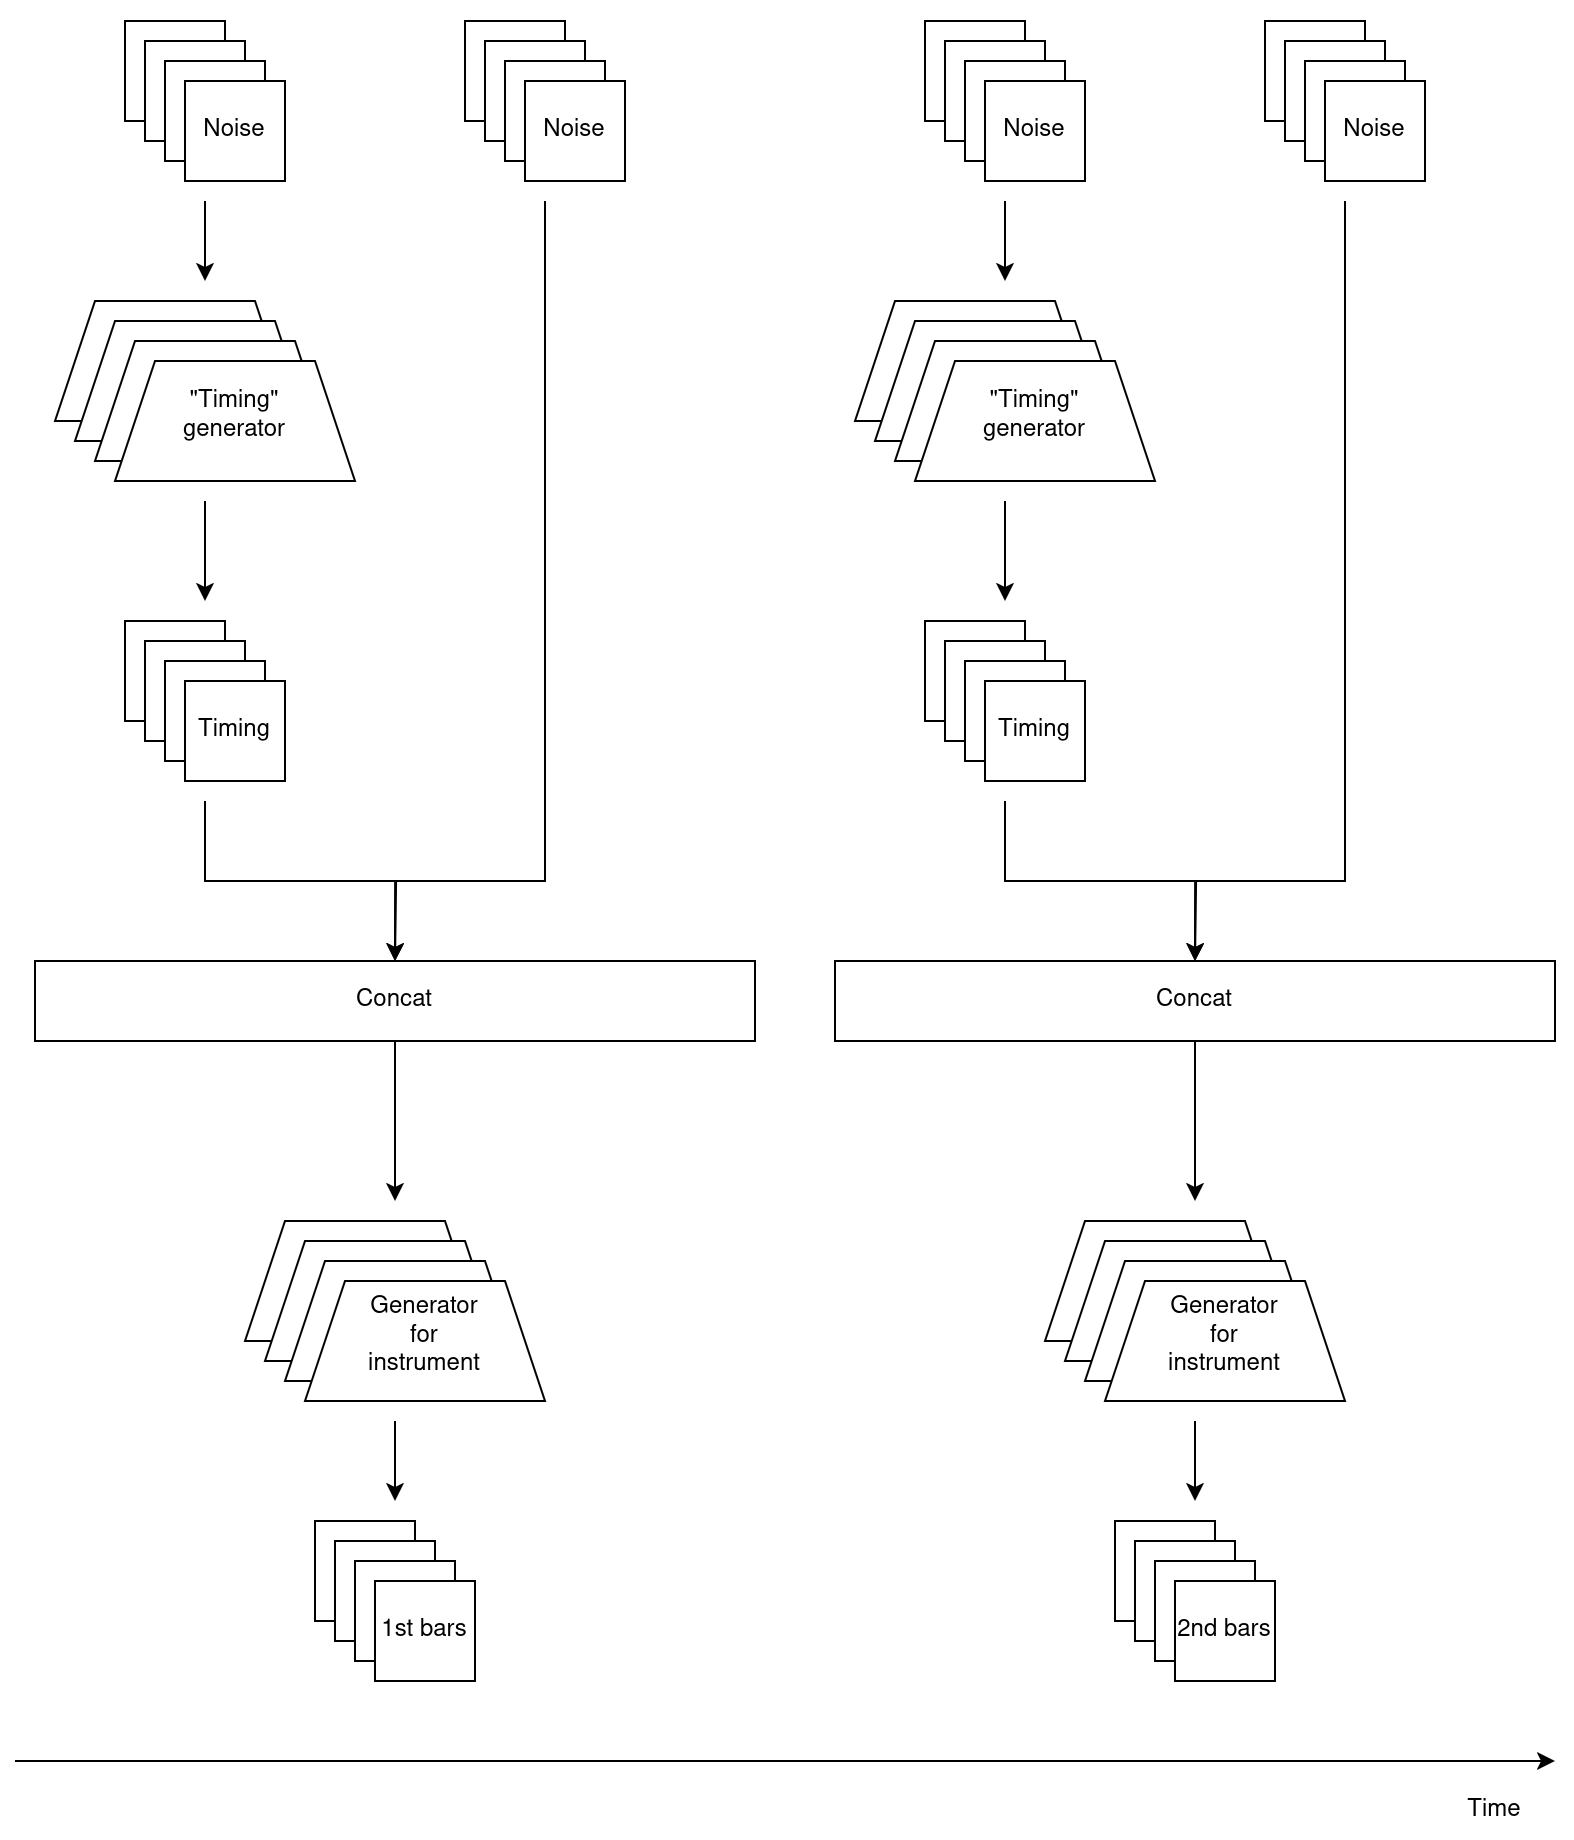
\includegraphics[height=8cm]{musegan.method.png}
    \caption{Inferența folosind MuseGAN}
    \label{musegan-method}
\end{figure}

\section{Music Transformer}

Huang et al. \cite{huang2018musictransformer} au propus un model bazat pe ``\textit{Transformere}''. Această arhitectură reușește să producă un rezultat semnificativ mai bun comparativ cu arhitecturile bazate pe LSTMuri. Pe parcursul cercetării, autorii au observat că gamele, arpegiile și alte motive muzicale exprimă o gramatică specifică unui compoziții muzicale și apar periodic în mod recurent. Această observație constituie motivația pentru utilizarea unui algoritm de ``\textit{Attention}'' relativ, algoritm ce permite captarea acestor relații.

Asemănător MusicGAN, modelul este antrenat pe un set de date public, compus din MIDIuri. Diferit însă de modelul precedent, datele sunt transformate în tokenuri discrete, tokenuri ce vor fi folosite în procesul de antrenare. Pe lângă datele tokenziate, modelul acceptă și niște tokenuri discrete pentru ritm și tempo.

\begin{figure}[H]
    \centering
    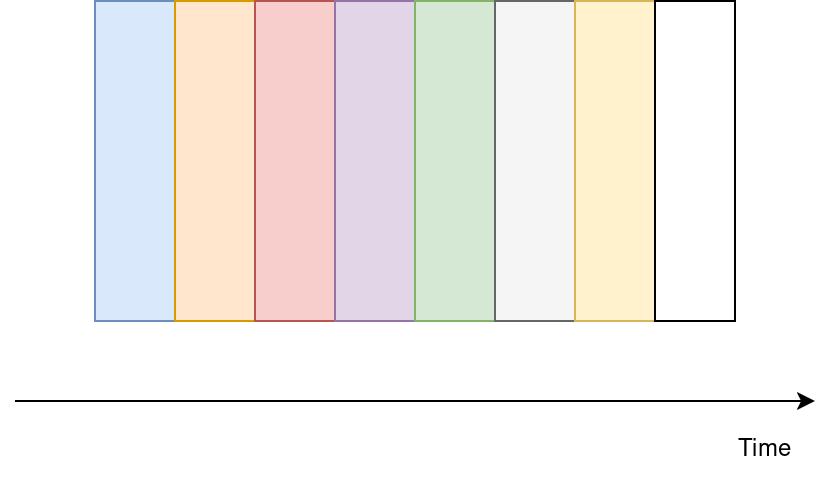
\includegraphics[height=5cm]{musictransformer.data.png}
    \caption{O secvență de tokenuri discrete}
    \label{music-transformer-data}
\end{figure}

La antrenare, modelul primește această secvență de tokenuri discrete. Modelul are drept sarcină să producă următorul token, folosind această secvență. Loss-ul generativ este reprezentat drept diferența dintre tokenul real și tokenul generat. Deoarece acest proces este realizat în acest mod, putem observa similarități cu seria de modele GPT \cite{radford2018improving}.

La inferență, modelul repetă procesul de antrenare: fiind oferită o secvență de tokenuri, modelul trebuie să genereze următorul token. După generarea acestuia, se realizează o alipire secvenței inițiale, iar procesul este repetat până când se obține durata solicitată.

\section{JukeBox}

Un alt model ce a reușit să împingă mai departe domeniul procesării și generării de muzică este ``\textit{JukeBox}'', propus de către Dhariwal et al. \cite{dhariwal2020jukeboxgenerativemodelmusic}. Modelul folosește o arhitectură de tipul ``auto-encoder variațional'' (VAE), cu straturi de tip ``Transformer'', formată dintr-un ``Encoder'' și un ``Decoder''.

Spre deosebire de modelele prezentate anterior, modelul folosește reprezentare sub formă de undă în mod direct. Acestea sunt eșantionate la 44.1KHz, și sunt segmentate în secvențe de 9-24 secunde.

La antrenare, primul nivel al ``Decoderului'' primește datele preprocesate, și produce tokenuri ``de dimensiuni mari''. Următoarele nivele (inclusiv ultimul nivel) primesc aceeași undă sonoră, respectiv tokenurile generate de către nivelele anterioare, producând astfel tokenuri din ce în ce mai granulare. Acest proces este asemănător unei rețele convoluționale ce are drept scop creșterea rezoluției unei imagini. Tokenurile finale sunt reprezentate într-un spațiu latent, spațiu în care informația este reprezentată într-un mod inteligibil pentru ``Decoder''. Rețeaua de ``Decoder'' primește drept date de intrare tokenii granulari din spațiul latent, și produc în final unde sonore. Pentru a evita o eventuală mapare a spațiului latent la doar o secțiune redusă de tokeni din codebook, autorii au ales să reinițializeze procesul de producere de embeddinguri.

\begin{figure}[H]
    \centering
    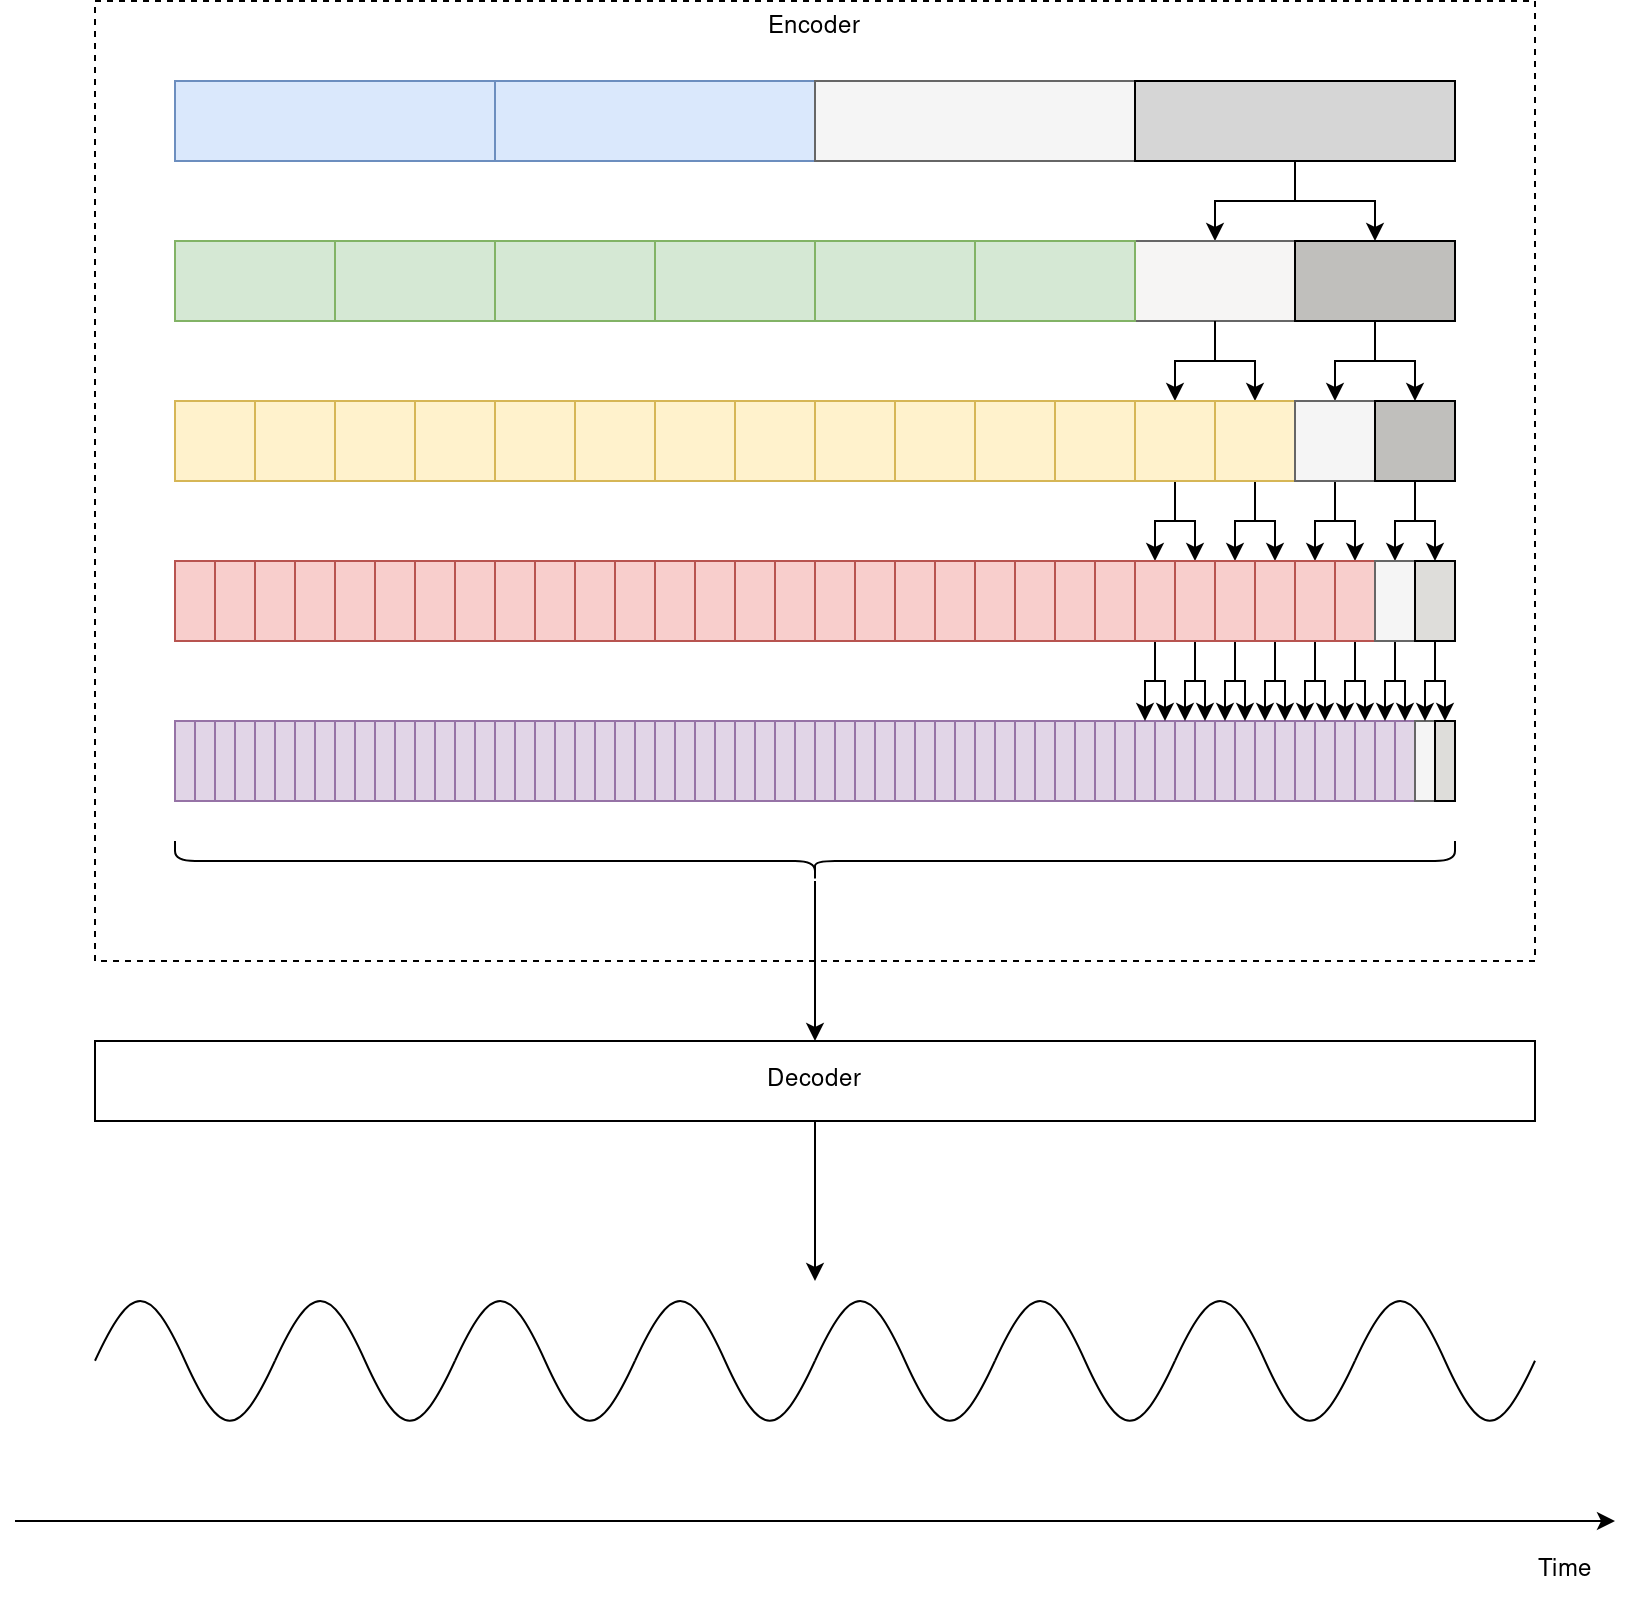
\includegraphics[height=10cm]{jukebox.architecture.png}
    \caption{Arhitectura modelului JukeBox}
    \label{jukebox-architecture}
\end{figure}

La inferență, partea de ``Encoder'' este eliminată, utilizatorul rețelei fiind capabil să folosească în mod direct tokenurile din spațiul latent.

\section{JEN}

JEN (Li et al.) \cite{li2025jen1textguideduniversalmusic} au propus un model ce folosește ``\textit{Diffusion}''. Acesta este capabil să primească text ca date de intrare cât și compoziții existente, și să le extindă sau să le modifice după instrucțiunile oferite. Modelul asigură o generare muzicală de calitate superioară, cu o bună coerență temporală și un control precis asupra stilului muzical dorit.

Modelul JEN-1 este antrenat pe ``un set de date care include 15.000 de piese muzicale licențiate de înaltă calitate, preluate de la Pond5''. Acestea sunt în format stereo la 48 kHz și conțin descrieri textuale, cât și etichete suplimentare pentru genul, instrumente, și stare. În preprocesare, semnalele audio sunt comprimate într-un spațiu latent continuu folosind un model de auto-encoder variațional (VAE) robust la zgomot. Acest VAE este antrenat cu obiective în domeniul temporal și frecvențial, evitând pierderile de calitate asociate cu cuantizarea.

Antrenarea JEN-1 se desfășură într-un cadru cu mai multe sarcini, având trei obiective principale: generarea muzicii din text (bidirecțional și unidirecțional), completarea muzicii (``inpainting''), și continuarea acesteia. Modelul este bazat pe un model ``UNet'' condiționat latent inspirat de ``Stable Diffusion'' (Rombach et al.) \cite{rombach2022highresolutionimagesynthesislatent}, care combină atenție autoregresivă și non-autoregresivă. În fiecare batch de antrenare, $\frac{1}{3}$ din date sunt alocate fiecărei sarcini. Pentru generarea condiționată, se folosește o strategie fără clasificator (classifier-free guidance), iar pentru a genera embeddingurile text este folosit ``\textit{FLAN-T5}'' (Chung et al.) \cite{huang2018musictransformer}.

În timpul inferenței, JEN-1 poate genera muzică folosindu-se de un prompt textual sau de un fragment muzical parțial (pentru ``inpainting'' sau continuare). Modelul permite comutarea între modul bidirecțional și unidirecțional fără a fi necesare modificări arhitecturale. Rezultatul este o piesă muzicală stereo de 48kHz ce reflectă promptul textual, cu o coerență melodică și armonică ridicată.
